\documentclass[a4paper,10pt]{article}

\usepackage{etex}
\reserveinserts{28}

\usepackage{xkeyval}[2005/11/25]
\usepackage{eso-pic}
\usepackage{graphicx}
\usepackage{fp}
\usepackage{tikz}
\usetikzlibrary{calc}
\usetikzlibrary{decorations.pathmorphing}
\usetikzlibrary{decorations.pathreplacing} 
\usetikzlibrary{decorations.shapes} 
\usetikzlibrary{shadows}
\usetikzlibrary{arrows}
\usetikzlibrary{shapes,snakes,shapes.geometric,shapes.misc}
\usepackage{multicol}
\usepackage{arabtex}
\usepackage{amsmath,amsfonts,amssymb}
\usepackage{float}
\usepackage{array,booktabs ,tabularx,multirow}
%\usepackage{euler}
\usepackage[top=1cm,bottom=0cm,left=1cm,right=1cm]{geometry}
\usepackage{fancyhdr}
\usepackage{xlop}
%\usepackage[most]{tcolorbox}
%----------------------------------------...les compteurs..... ----------------------------------------------------------------------%
\newcounter{i}
\setcounter{i}{1}
\newcounter{k}
\setcounter{k}{1}
%----------------------------------------------------------\cadre[x=... ,y=.....,  ]------------------------------------------------------%

% \cadre[			shadow (bool�en),
%					lw = , (�paisseur du trait, en pt)
%					style = , (dashed ou dotted)
%					x = abscisse du sommet en bas � gauche,
%					y = ordonn�e du sommet en bas � gauche,
%					xshadow = d�calage selon x de l'ombre,
%					yshadow = d�calage selon y de l'ombre,
%					color = couleur du cadre,
%					colorshadow = couleur de l'ombre,
%					decoration = nom de la d�coration,
%					doubleline (bool�en) pour pstricks
%				  ]
\makeatletter
\define@cmdkey [PAS] {cadre} {x}{}
\define@cmdkey [PAS] {cadre} {y}{}
\define@cmdkey [PAS] {cadre} {decoration}{}
\define@cmdkey [PAS] {cadre} {shape}{}
\define@cmdkey [PAS] {cadre} {lw}{}
\define@cmdkey [PAS] {cadre} {xshadow}{}
\define@cmdkey [PAS] {cadre} {yshadow}{}
\define@cmdkey [PAS] {cadre} {bordercolor}{}
\define@cmdkey [PAS] {cadre} {incolor}{}
\define@cmdkey [PAS] {cadre} {shadowcolor}{}
\define@cmdkey [PAS] {cadre} {style}{}
\define@boolkey[PAS] {cadre} {shadow}[true]{}
\define@boolkey[PAS] {cadre} {doubleline}[true]{}

\presetkeys    [PAS] {cadre} {	shadow = false,
								lw = 2,
								x = 0.2,
								y = 0.2,
								xshadow =- 0.35,
								yshadow =0.2,
								bordercolor = black,
								incolor = white,
								shadowcolor = gray,
								style = ,
								doubleline = false,
								decoration = , 
								shape = }{}

\newcommand*{\cadre}[1][]{\pasCadre[#1]}

\def\pasCadre[#1]{
	\setkeys[PAS]{cadre}{#1}
	
	\AddToShipoutPicture
	{
		\put(\LenToUnit{\cmdPAS@cadre@x cm},\LenToUnit{\cmdPAS@cadre@y cm})
		{
				\ifPAS@cadre@doubleline
					\edef\dl{double}
				\else
					\edef\dl{}
				\fi
				\begin{tikzpicture}[decoration={\cmdPAS@cadre@decoration,shape=\cmdPAS@cadre@shape}]
					\pgfsetlinewidth{\cmdPAS@cadre@lw pt}
					\ifPAS@cadre@shadow
						\filldraw[
						decorate,
						fill=\cmdPAS@cadre@incolor,
						draw=\cmdPAS@cadre@bordercolor,
						style=\cmdPAS@cadre@style,
						drop shadow={fill=\cmdPAS@cadre@shadowcolor,shadow xshift=\cmdPAS@cadre@xshadow cm,shadow yshift=-\cmdPAS@cadre@yshadow cm},
						\dl] (0,0) -- (0,\paperheight-2*\cmdPAS@cadre@y cm) -- (\paperwidth-2*\cmdPAS@cadre@x cm,\paperheight-2*\cmdPAS@cadre@y cm) -- (\paperwidth-2*\cmdPAS@cadre@x cm,0) -- cycle;
					\else
						\filldraw[
						decorate,
						fill=\cmdPAS@cadre@incolor,
						draw=\cmdPAS@cadre@bordercolor,
						style=\cmdPAS@cadre@style,
						\dl] (0,0) -- (0,\paperheight-2*\cmdPAS@cadre@y cm) -- (\paperwidth-2*\cmdPAS@cadre@x cm,\paperheight-2*\cmdPAS@cadre@y cm) -- (\paperwidth-2*\cmdPAS@cadre@x cm,0) -- cycle;
					\fi
				\end{tikzpicture}
		}
	}
}

\def\nocadre{\ClearShipoutPicture}
%-----------------------------------------------\entete---------------------------------------------------------------------------%
\newcommand{\entete}{
\noindent
\begin{tabularx}{\textwidth}{|r  ||||X|||| r |}
\toprule
\RL{AlmdT AlzmnyT : $1 H$}
&
\centering \RL{{\LARGE Altqwym Alt^sxy.sy }}
&
 \RL{Al-'ism : \hspace{4cm}}\\
 \RL{AldwrT : $I$}& \centering   \RL{\Large{fy m|AdT AlryA.dyAt}}&\RL{Alnq.tT } \\
 \RL{Alm`Aml : $3$} & \centering  \RL{AlsnT Al_tAl_tT 'i`dAdy} & \\
 \bottomrule
\end{tabularx}
}
%-----------------------------------------------
\newcommand{\ExamEntete}{
\noindent
\begin{tabularx}{\textwidth}{||r  ||||X|||| c ||}
\toprule \toprule
\begin{minipage}{0.2\textwidth}
\centering\includegraphics[scale=1]{../images/nourQamar.png}

\begin{arabtext}
AlmdT AlzmnyT : sA`T 

dwrT : ynAyr $2019$

Alm`Aml : $1$
\end{arabtext}
\end{minipage}&
\begin{minipage}{0.4\textwidth}
\begin{center}
 \RL{{\LARGE Alfr.d Almnzly $1$ fy AlryA.ayAt  }}

\RL{\Large{fy mAdT AlryA.dyAt}}

 \RL{AlsnT Al_tAl_tT 'i`dAdy } 
 \end{center}
\end{minipage}&
\begin{minipage}{0.3\textwidth}
\centering\includegraphics[scale=0.5]{images/logo.jpg}
\end{minipage}\\
 \bottomrule  \bottomrule
\end{tabularx}
}
%--\exercice[bareme,bar=...]{........}------------------------------%
\define@cmdkey[EX]{exo}{bar}{}
\define@boolkey[EX]{exo}{bareme}[true]{}
\presetkeys[EX]{exo}{bar= ,bareme=false}{}
\newcommand{\exercice}[2][]{
\setkeys[EX]{exo}{#1}
\setcounter{k}{1}
\tikzstyle{mybox} = [ draw, very thick,rounded corners=3mm, inner sep=10pt, inner ysep=10pt]
\tikzstyle{fancytitle} =[fill=white, text=black,inner ysep=0pt,inner xsep=2pt]
\noindent
\begin{tikzpicture}
\node [mybox] (box){%
    \begin{minipage}{0.88\linewidth}
        #2 
    \end{minipage}
};
\node[fancytitle, right=10pt] at (box.north west) {{\large \LR{Exercice}\arabic{i}}};
\ifEX@exo@bareme
\node[fancytitle] at (box.north){ \cmdEX@exo@bar \LR{pts}};
\fi
\end{tikzpicture}%
\stepcounter{i}
}
%-----------\question[bareme,bar=...]{......}----------------------%
\define@cmdkey[EX]{qst}{bar}{}
\define@boolkey[EX]{qst}{bareme}[true]{}
\presetkeys[EX]{qst}{bar= ,bareme=false}{}
\newcommand{\question}[2][]{
\setkeys[EX]{qst}{#1}
\ifEX@qst@bareme
	\ifdim \cmdEX@qst@bar pt  < 2 pt
\begin{arabtext}
$-\arabic{k}$ \marginpar{ \cmdEX@qst@bar{} pt} #2
\end{arabtext}
	\else
\begin{arabtext}
$-\arabic{k}$ \marginpar{ \cmdEX@qst@bar{} pts} #2
\end{arabtext}
	\fi
\else
\begin{arabtext}
$-\arabic{k}$ #2
\end{arabtext}
\fi
\stepcounter{k}
}
%----------\devoirp[niv=... , num=..., date=..., ds=...]----------%
\define@cmdkey[EX]{devoir}{ds}{}
\define@cmdkey[EX]{devoir}{niv}{}
\define@cmdkey[EX]{devoir}{num}{}
\define@cmdkey[EX]{devoir}{date}{}
\presetkeys[EX]{devoir}{niv=$3$,num=$1$,ds=,date=}{}
\newcommand{\devoir}[1][]{
\setkeys[EX]{devoir}{#1}
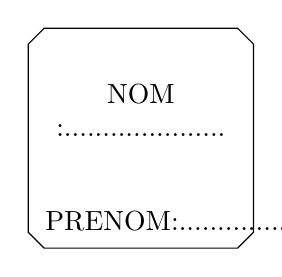
\begin{tikzpicture}
\node [draw,shape=chamfered rectangle] (box1){%
    \begin{minipage}{0.2\textwidth}
    \vspace{0.5cm}
  \center  NOM :.....................
    
   \center PRENOM:...................  
    \end{minipage}
};
\end{tikzpicture}%
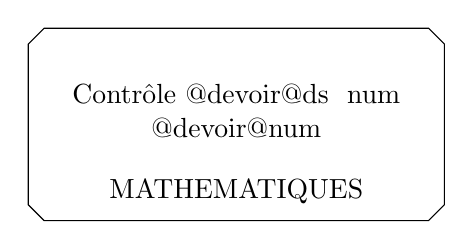
\begin{tikzpicture}
\node [draw,shape=chamfered rectangle] (box2){%
    \begin{minipage}{0.4\textwidth}
    \vspace{0.5cm}
       \center Contrôle \cmdEX@devoir@ds {} num \cmdEX@devoir@num  
           
        \center MATHEMATIQUES
    \end{minipage}
};
\end{tikzpicture}%
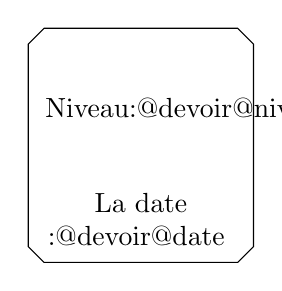
\begin{tikzpicture}
\node [draw,shape=chamfered rectangle] (box3){%
    
    \begin{minipage}{0.2\textwidth}
    \vspace{0.5cm}
    \center\LR{Niveau:{}\cmdEX@devoir@niv  } 
    
      \center  \LR{La date :{}\cmdEX@devoir@date }
    \end{minipage}
};
\end{tikzpicture}%
}
%------------------------------------------------\serie[titre=..]-----------------------------------------------------------------------------%

\define@cmdkey[EX]{serie}{titre}{}
\presetkeys[EX]{serie}{titre=\RL{`nwAn Aldrs}}{}
\newcommand{\serie}[1][]{
\setkeys[EX]{serie}{#1}
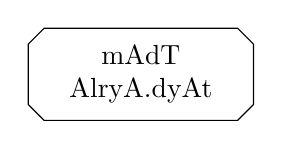
\begin{tikzpicture}
\node [draw,shape=chamfered rectangle] (box1){%
    \begin{minipage}{0.20\textwidth}
       \center\RL{mAdT AlryA.dyAt}
    \end{minipage}
};
\end{tikzpicture}%
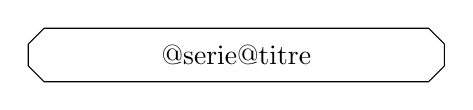
\begin{tikzpicture}
\node [draw,shape=chamfered rectangle] (box2){%
    \begin{minipage}{0.40\textwidth}
      \center\cmdEX@serie@titre
    \end{minipage}
};
\end{tikzpicture}%
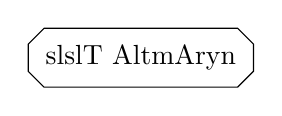
\begin{tikzpicture}
\node [draw,shape=chamfered rectangle] (box3){%
    \begin{minipage}{0.20\textwidth}
   \center\RL{slslT AltmAryn}
    \end{minipage}
};
\end{tikzpicture}%
}
\makeatother

%\cadre[x=0.5,y=0.1,doubleline]

\pagestyle{empty}
\begin{document}
\begin{tabular}{|p{0.25\linewidth 
}|p{0.4\linewidth }| p{0.25\linewidth }|}
\hline
\begin{center}
\RL{dwrT ynAyr $2017$}
\end{center} &
\begin{center}
\RL{`nA.sr 'ijAbT Al-'imt.hAn Almw.hd Alm.hly fy AlryA.dyAt}
\end{center}&
\begin{center}
 \RL{ Al_tAnwyT Al-'i`dAdyT AlrAzy }
\end{center}  \\ 
\hline 
\end{tabular} 
\begin{multicols}{2}[\RLmulticolcolumns,\raggedcolumns,\setlength{\columnsep}{1 cm}]
\exercice[bar=6,bareme]{
\question[bareme,bar=2]{A.hsb  : $ a=\sqrt{81}=9\quad$ w $\quad  b=\dfrac{\sqrt{27}}{\sqrt{3}}=\sqrt{\dfrac{27}{3}}=\sqrt{9}=3\quad $ w $\quad c=(3+\sqrt{5})(3-\sqrt{5})=3^{2}-\sqrt{5}^{2}=4$} 
\question[bareme,bar=1]{bs.t :
$\quad d=\sqrt{18}-\sqrt{8}=3\sqrt{2}-2\sqrt{2}=\sqrt{2} $ w
$\quad e=\sqrt{6+\sqrt{5}}\times \sqrt{6-\sqrt{5}}=\sqrt{6^{2}-5}=\sqrt{31}$
}
 \question[bareme,bar=2]{'uktb `lY ^skl qwT : \hspace{1cm} 
  $\ y=6^{31}\times 5^{31}=30^{31} $ w $\quad  z=(3^{2})^{8}\times (27)^{6}=3^{34}$  }
 \question[bareme,bar=1]{`ml :\hspace{1cm} 
$A= (x+1)(2x-1)+2x+2=(x+1)(2x+1)$ \hspace{1cm}  w
$B=4x^{2}-4x+1=(2x-1)^{2}$
 }
}

\exercice[bar=4,bareme]{
\question[bareme,bar=1]{qArn Al`dadyn : $4\sqrt{3}$ w $5\sqrt{2}$}
\begin{arabtext}
ldynA $(4\sqrt{3})^{2}=48$ w $(5\sqrt{2})^{2}=50$ 'i_dn $5\sqrt{2}\geq 4\sqrt{3}$
\end{arabtext}
\question[bareme,bar=3]{$x$ w $y$  `dadAn .hqyqyAn  b.hy_t $3 \leq x \leq 7$ w $4 \leq y \leq 5$.

 'a.tr mA yly : $\quad x+y$ w $\quad 3x-y$ w $\quad \dfrac{x}{y}$}

\begin{arabtext}
\center
$7 \leq x+y\leq 12$

$4\leq 3x-y \leq 17$

$\dfrac{3}{5}\leq\dfrac{x}{y}\leq \dfrac{7}{4}$
\end{arabtext}
}

\exercice[bar=3,bareme]{
\begin{minipage}{0.4\linewidth}
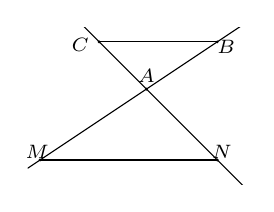
\begin{tikzpicture}[scale=0.5,line cap=round,line join=round,>=triangle 45,x=1.0cm,y=1.0cm,scale=0.75]
\clip(-3.42,0.18) rectangle (3.96,5.48);
\draw [domain=-3.42:3.96] plot(\x,{(--16-4*\x)/4});
\draw [domain=-3.42:3.96] plot(\x,{(-18-4*\x)/-6});
\draw (-1,5)-- (3,5);
\draw (-3,1)-- (3,1);
\begin{scriptsize}
\fill [color=black] (-1,5) circle (1.5pt);
\draw[color=black] (-1.64,4.9) node {$C$};
\fill [color=black] (3,1) circle (1.5pt);
\draw[color=black] (3.16,1.28) node {$N$};
\fill [color=black] (3,5) circle (1.5pt);
\draw[color=black] (3.3,4.84) node {$B$};
\fill [color=black] (-3,1) circle (1.5pt);
\draw[color=black] (-3.1,1.28) node {$M$};
\fill [color=black] (0.6,3.4) circle (1.5pt);
\draw[color=black] (0.6,3.86) node {$A$};
\end{scriptsize}
\end{tikzpicture}
\end{minipage}
\begin{minipage}{0.6\linewidth}
\begin{arabtext}
n`tbr Al^skl jAnbh b.hy_t $AB=4$ w $AC=2$ w  $AM=6$ w $AN=3$
\end{arabtext}
\question[bareme,bar=1.5]{byn 'anna Almstqymyn $(MN)$ w $(BC)$ mtwAzyAn }
\end{minipage}
\begin{arabtext}
ldynA $A\in [BM]$ w $A\in [CN]$ w $\dfrac{AB}{AM}=\dfrac{4}{6}=\dfrac{2}{3}$ w$\dfrac{AC}{AN}=\dfrac{2}{3}$

'i_dn $\dfrac{AB}{AM}=\dfrac{AC}{AN}$ w bmA anna Alnq.t $B$ w $A$ w $M$ fy nfs Altrtyn m` $C$ w $A$ w $N$ fa-'in .h m .t ` AlmstqymAn $(MN)$ w $(BC)$ mtwAzyAn .
\end{arabtext}
\question[bareme,bar=1.5]{'i_dA `lmt 'anna $BC=5$ fA.hsb $MN$ }
\begin{arabtext}
ldynA $(MN)//(BC)$ .h m .t m 
$$\dfrac{AC}{AN}=\dfrac{AB}{AM}=\dfrac{BC}{MN}$$
'i_dn $MN=\dfrac{BC \times AM}{AB}=\dfrac{30}{4}=7.5$
\end{arabtext}
}

\exercice[bar=5,bareme]{
\begin{minipage}{0.3\linewidth}
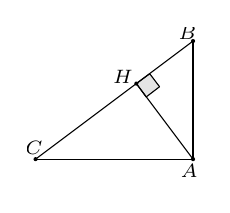
\begin{tikzpicture}[scale=0.5,line cap=round,line join=round,>=triangle 45,x=1.0cm,y=1.0cm,rounded corners=0pt,scale=1]
\clip(-2.2,0.36) rectangle (2.22,4.34);
\draw[color=black,fill=black,fill opacity=0.1] (0.81,2.58) -- (1.15,2.84) -- (0.9,3.17) -- (0.56,2.92) -- cycle; 
\draw (2,1)-- (2,4);
\draw (2,4)-- (-2,1);
\draw (-2,1)-- (2,1);
\draw (2,1)-- (0.56,2.92);
\begin{scriptsize}
\fill  (2,1) circle (1.5pt);
\draw (1.9,0.7) node {$A$};
\fill  (2,4) circle (1.5pt);
\draw (1.86,4.2) node {$B$};
\fill  (-2,1) circle (1.5pt);
\draw (-2.04,1.28) node {$C$};
\fill  (0.56,2.92) circle (1.5pt);
\draw (0.22,3.08) node {$H$};
\end{scriptsize}
\end{tikzpicture}
\end{minipage}\hfill
\begin{minipage}{0.7\linewidth}
\begin{arabtext}
$.I$n`tbr Al^skl jAnbh b.hy_t : $AB=2$w $AC=4$w$BC=2\sqrt{5}$
\end{arabtext}
\question[bareme,bar=1]{byn 'anna Alm_tl_t $ABC$ qA'im AlzAwyT fy $A$}
\end{minipage}
\begin{arabtext}
ldynA $BC^{2}=AB^{2}+AC^{2}$ .h m f m Alm_tl_t $ABC$ qA'im AlzAwyT fy $A$ .
\end{arabtext}
\question[bareme,bar=1.5]{'u.hsb $cos\widehat{ABC}$w$sin\widehat{ABC}$w $tan\widehat{ABC}$} 
\begin{arabtext}
$$\cos\widehat{B}=\dfrac{\sqrt{5}}{5};;
\sin\widehat{B}=\dfrac{2\sqrt{5}}{5} ;;
\tan\widehat{B}=2 $$
\end{arabtext}
\question[bareme,bar=1]{ ltkn $H$ Almsq.t Al`mwdy lilnq.tT $A$ `lY $[BC]$. 'u.hsb $BH$ }
\begin{arabtext}
n`tbr Alm_tl_t $ABH$. $\cos\widehat{B}=\dfrac{BH}{AB}=\dfrac{\sqrt{5}}{5}$

$$BH=\dfrac{2\sqrt{5}}{5}$$
\end{arabtext}
\begin{arabtext}
$.II$ ltkn $a$ qyAs zAwyT .hAdT , .hy_t $\sin a=\dfrac{1}{5}$.
\end{arabtext}
\question[bareme,bar=1]{ A.hsb $\cos a$ w $\tan a$ .}
\begin{arabtext}
$$\cos^{2} a=1-(\dfrac{1}{5})^{2}=\dfrac{24}{25} \Rightarrow \cos a =\dfrac{\sqrt{24}}{5} $$
$$\tan a= \dfrac{1}{5}\div\dfrac{\sqrt{24}}{5}=\dfrac{1}{\sqrt{24}} $$
\end{arabtext}
\question[bareme,bar=0.5]{byn anna : $\dfrac{tan20^{\circ}}{1+tan20^{\circ}}-\dfrac{1}{1+tan70^{\circ}}=0$}
$$\dfrac{tan20^{\circ}}{1+tan20^{\circ}}=\dfrac{\dfrac{1}{tan70^{\circ}}}{1+\dfrac{1}{tan70^{\circ}}}=\dfrac{1}{1+tan70^{\circ}} $$
}

\exercice[bar=2,bareme]{
\begin{minipage}{0.3\linewidth}
\definecolor{uuuuuu}{rgb}{0.27,0.27,0.27}
\definecolor{cqcqcq}{rgb}{0.75,0.75,0.75}
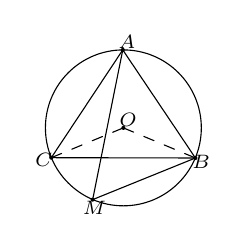
\begin{tikzpicture}[scale=0.5,line cap=round,line join=round,>=triangle 45,x=0.75cm,y=0.75cm]
\draw(-1,3) circle (1.98cm);
\draw (-1.02,5.64)-- (-3.44,1.99);
\draw (-1.02,5.64)-- (1.44,1.98);
\draw (1.44,1.98)-- (-3.44,1.99);
\draw [dash pattern=on 4pt off 4pt] (-3.44,1.99)-- (-1,3);
\draw [dash pattern=on 4pt off 4pt] (-1,3)-- (1.44,1.98);
\draw (-1.02,5.64)-- (-2.04,0.57);
\draw (-2.04,0.57)-- (1.44,1.98);
\begin{scriptsize}
\fill [color=black] (-1,3) circle (1.5pt);
\draw[color=black] (-0.84,3.28) node {$O$};
\fill [color=black] (1.44,1.98) circle (1.5pt);
\draw[color=black] (1.64,1.86) node {$B$};
\fill [color=black] (-1.02,5.64) circle (1.5pt);
\draw[color=black] (-0.88,5.92) node {$A$};
\fill [color=black] (-3.44,1.99) circle (1.5pt);
\draw[color=black] (-3.7,1.9) node {$C$};
\fill [color=black] (-2.04,0.57) circle (1.5pt);
\draw[color=black] (-1.98,0.3) node {$M$};
%\fill [color=uuuuuu] (-1.76,1.98) circle (1.5pt);
%\draw[color=uuuuuu] (-1.6,1.7) node {$I$};
\end{scriptsize}
\end{tikzpicture}
\end{minipage}\hfill
\begin{minipage}{0.7\linewidth}
\begin{arabtext}
fy Al^skl jAnbh ldynA $(C)$ dA'irT mrkzhA $O$ m.hy.tT bm_tl_t $ABC$ mtsAwy AlsAqyn fy $A$ b.hy_t $\widehat{BAC}=70^{\circ}$ .
\end{arabtext}
\end{minipage}
\question[bareme,bar=1]{.hdid  qyAs AlzAwyT $\widehat{BOC}$}
$$\widehat{BOC}=2\widehat{BAC}=140^{\circ} $$
\question[bareme,bar=1]{.hdid qyAs AlzAwyT : $\widehat{AMB}$}
$$\widehat{AMB}=\widehat{ACB}=\dfrac{180^{\circ}-70^{\circ}}{2}=55^{\circ} $$
}



\end{multicols}
\end{document}